\documentclass[conference]{IEEEtran}
\IEEEoverridecommandlockouts
\usepackage{cite}
\usepackage{amsmath,amssymb,amsfonts}
\usepackage{algorithmic}
\usepackage{graphicx}
\usepackage{textcomp}
\usepackage{listings}
\usepackage{graphicx}
\graphicspath{ {images/} }
\def\BibTeX{{\rm B\kern-.05em{\sc i\kern-.025em b}\kern-.08em
    T\kern-.1667em\lower.7ex\hbox{E}\kern-.125emX}}

\title{\#4 Assignment - Implementing Scientific Computations - CMPT 383}
\author{Luiz Fernando Peres de Oliveira - 301288301 - lperesde@sfu.ca}
\date{October 27th, 2017}
\begin{document}
\maketitle
\section{Introduction}
Numerical methods for scientific problems, especially in engineering and science, are frequently related to solving problems for large matrices (such as image processing). Many of the most efficient algorithms for large-scale matrix computations are based on approximations of the given matrix by small matrices (e.g. kernel convolution and Petrov-Galerkin projections).
\\\\
Traversing matrices is one of the heaviest numerical computations as, for a given matrix \textbf{m} with \textit{r} rows and \textit{c} columns, it has known time complexity of $O(r\times c)$. Imagine that we have a bitmap image \textbf{img} of size $800 \times 600$ with \textit{RGB} colors, for example. Now imagine that we want to convert \textbf{img} into its grayscale representation.  In that case, it would take a time of $800 \times 600 \times 3$ (we multiply by 3 because we must consider the space occupied by $red$, $green$ and $blue$ values of each pixel) to traverse and convert every RGB pixel of \textbf{img} into its grayscale representation.
\\\\
The work below will discuss and illustrate how efficiently different paradigms use matrices to solve a given problem. The paradigms used will be \textit{(Functional Programming (Haskell), Object-oriented Programming (Java), Scripting Language (Python), Imperative Programming (Go) and Procedural Programming(C))}. For each paradigm here discussed, the programs are expected to vary in time complexity to traverse and apply map functions to matrices for large inputs as well as vary in resources (memory) allocation, as some paradigms might take more memory than others.
\\\\
Finally, it will be implemented, evaluated and discussed the map functions \textbf{add}, \textbf{multiply} and \textbf{custom} for each paradigm/language described above. Each one of these map functions take a \textit{matrix} \textbf{m} as input and return a \textit{matrix} \textbf{m'} as output. They can be represented mathematically as:

\begin{itemize}
	\item \textbf{add}: $c_{ij} = a_{ij} + b_{ij}$
	\item \textbf{multiply}: $c_{ij} = a_{ik} \times b_{kj}$
	\item \textbf{custom}: $c_{ij} = max(a_{ij}, b_{ij}) + a_{ij}^2 + b_{ij}^2$
\end{itemize}

\section{Related Work, Background and Applications}
Representation Theory is the field of study that uses matrices representations for problem solving  $[19]$. All finite groups can be represented as matrices, and, therefore, matrices are a very useful tool for studying finite groups.
\\\\
There are numerous applications in which matrices are a useful for scientific programming. For instance, matrices are largely used in the field of linear systems as a mean to represent and manipulate finite dimensional vector spaces. Matrices are are also very important in the field of linear algebra which is one of the most crucial tools in math. Some real-world applications for matrices are:  

\begin{itemize}
	\item \textbf{Computer Graphics and Image Processing}: Your computer graphics are represented by matrices. The major task of the \textit{GPU} is to calculate more than a billion matrix operations per second. Also, reflection and distortion effects applied on images such as the Gaussian and Sobel operators are represented by matrices as well as the images themselves.
	\item \textbf{Linear systems arithmetic}: Linear systems take advantage of matrix arithmetic. For instance, error-correcting codes and linear differential equations.
	\item \textbf{Supports Graph Theory}: Graphs may be abstracted as matrices.
	\item \textbf{Probability and Statistics}: The field of probability and statistics use matrix representations such as probability vectors of a neural system and Markov Chains on stochastic matrices.
	\item \textbf{2D and 3D Geometry}: Matrices 
\end{itemize}

That is to say, scientific programming is related to many fields and therefore it is not possible to describe completely its current \textit{state of the art}. Current work on scientific programming using matrices focus in Computer Graphics, Geometry and problem solving in general. For more details on current work on scientific programming with matrices, please check $[21]$, $[22]$, $[23]$ and $[24]$. Note that the given references are only examples and therefore, they do not represent all works on the large field of scientific programming). 

\section{Implementation}

\textbf{ Object-oriented Programming - Java }\\
The way Object-oriented programming paradigm behaves regarding scientific programming can be related to the Object-oriented language we are using, because such paradigm is often implemented in multi-paradigm languages. For example, \textit{Java, Erlang, Objective-C and Pony} will most likely have different ways and use different methods for processing numerical computations. That happens because these languages are not only Object-oriented, but also imperative (for Java and Objective-C) and Process-Calculus-based(Erlang and Pony), a paradigm very close to Functional Programming, where "everything" is a process rather than a function. That is to say, Java will be representative language for this category, but what is true to Java might \textbf{not} be true to other different \textit{OOP languages}.
\\\\
Java is one of the \textit{C-family} languages$[11]$ and for this reason, scientific programming in pure Java can be \textbf{very} similar to scientific programming in C (not accounting direct access to pointers). In fact, it would be very hard to identify and distinguish scientific programs in pure Java or/and in pure C (not considering classes and particularities of the Object-oriented paradigm).
\\\\
Java has the benefit of having multiple frameworks for numerical computations, such as \textit{COLT, JLAPACK, ND4J, Matrix toolkit Java} and others. However, I chose to write numerical computations in pure Java for this assignment, as I would like to compare it with C (because the code is very similar, but there might be differences in runtime because of the different compilers for these languages and because Java's bytecode will be interpreted by the JVM). 
\\
On the code snippets below, you will see how one would represent the map functions \textbf{add}, \textbf{multiply} and \textbf{custom} in Java.
\\
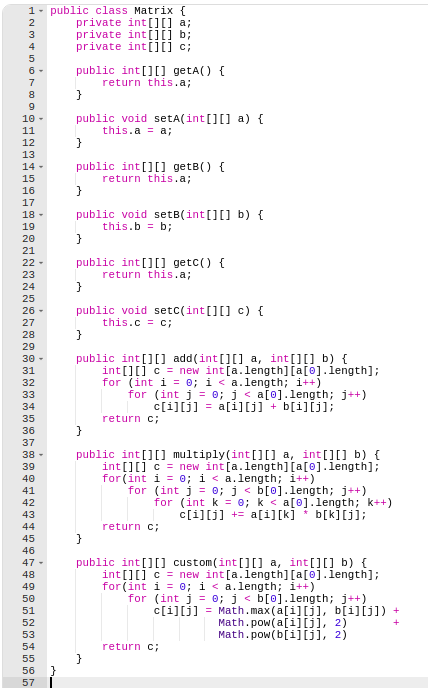
\includegraphics[scale=0.57]{java_code}

The previous Java code will traverse matrices as fast as C would do and in fact (with limitations on the JVM), it is very hard to distinguish the differences between that code and a given C code for the same task. You can of course see that the Java code is very verbose regarding such simple functions. In order to execute the code, we will need to have a \textit{Java class} that implements the \textit{main} function. In this way, our class will be instantiated into an object of type \textbf{Matrix} and only them, after setting it up properly, we would be able to use all the power of this language. Also, this Java code allows us to use custom sizes for our data $d$ described on the introduction 

\textbf{ Functional Programming - Haskell }

Functional programming in general appears to have many beautiful ways of traversing matrices, given (in theory) the lack of side effects and its foundation of applying mathematical functions to the real world, however, in practice, this may not work as beautiful as it seems because a bigger problem may be divided into many small problems (function calls, as high order functions are always broken down in other smaller functions), which may impact on the speed of a given program, once that it would be faster if the process was done linearly$[5]$ (the way that imperative languages would try to solve this category of problems). Haskell will be the representative of the Functional Programming paradigm for this assignment.
\\\\
On the code below, you will see how one would represent the map functions \textbf{add}, \textbf{multiply} and \textbf{custom} in Haskell.



\textbf{CODE HERE}

\textbf{ Scripting Language - Python }
As said before on previous assignments, scripting languages usually run slower than compiled languages (because of the time that is spent on just-in-time translations). Python has a slight advantage on other scripting languages because it uses many libraries written in pure C, boosting the process of interpreting programs.
\\\\
Python is multi-paradigm and allows \textbf{imperative programming} as well, just like \textit{Fortran, Java and C} and is reasonable to think that it will be one of fastest languages for this assignment. One point is that it is well known as a scientific programming language with numerous libraries out there, such as \textit{NumPy} (which is mostly written in C). Lastly, Python allows "hacks" for performance when dealing with matrix handling. For this assignment, it was chosen to use \textit{NumPy} for scientific programming.
\\\\
The code below takes bitmap image as input and outputs its grayscale representation:

\lstset{language=python}
\begin{lstlisting}[frame=single]
import numpy as np

def rgb2gray(rgb):
    return np.dot(rgb[...,:3],
      [0.299, 0.587, 0.114])

img = mpimg.imread(filename)     
grayimg = rgb2gray(img)    
mpimg.imsave(filename, grayimg)
\end{lstlisting}

Compared to all other seen snippets, so far, Python is the one with clearest code and helps us understand why the scientific community enforce the use of this tool. We still need to check how fast it is indeed (in comparison with other programming paradigms and languages, such as \textit{Fortran and Java}).

\section{Results}

\section{Discussion}

\begin{thebibliography}{00}
\bibitem{b1} "IWASEP", 2017. [Online]. Available: http://www4.ncsu.edu/~ipsen/ps/slides\_iwasep.pdf. [Accessed: 28- Oct- 2017].

\bibitem{b2} "Freund\_HLA", 2017. [Online]. Available: https://www.math.ucdavis.edu/~freund/freund\_HLA.pdf. [Accessed: 28- Oct- 2017].

\bibitem{b3} "Big O notation", En.wikipedia.org, 2017. [Online]. Available: https://en.wikipedia.org/wiki/Big\_O\_notation. [Accessed: 28- Oct- 2017].

\bibitem{b4} "Tweag I/O - Enter the matrix, Haskell style", Tweag.io, 2017. [Online]. Available: https://www.tweag.io/posts/2017-08-31-hmatrix.html. [Accessed: 28- Oct- 2017].

\bibitem{b5} "Functional vs. Imperative Programming", Ryanhmckenna.com, 2017. [Online]. Available: http://www.ryanhmckenna.com/2014/11/functional-vs-imperative-programming.html. [Accessed: 28- Oct- 2017].

\bibitem{b6} "hmatrix", 2017. [Online]. Available: http://dis.um.es/~alberto/material/hmatrix.pdf. [Accessed: 28- Oct- 2017].

\bibitem{b7} "For scientific computing, is Java useful in a way that C or Python aren't? - Quora", Quora.com, 2017. [Online]. Available: https://www.quora.com/For-scientific-computing-is-Java-useful-in-a-way-that-C-or-Python-arent. [Accessed: 28- Oct- 2017].

\bibitem{b8} "Scientific Computation", Introcs.cs.princeton.edu, 2017. [Online]. Available: https://introcs.cs.princeton.edu/java/90scientific/. [Accessed: 28- Oct- 2017].

\bibitem{b9} "Java And Cpp Platforms For Scientific Computing", 2017. [Online]. Available: https://inside.mines.edu/~dhale/papers/Hale06JavaAndCppPlatformsForScientificComputing.pdf. [Accessed: 28- Oct- 2017].

\bibitem{b10} P. Knoll and S. Mirzaei, "Scientific computing with Java", 2017.

\bibitem{b11} "List of C-family programming languages", En.wikipedia.org, 2017. [Online]. Available: https://en.wikipedia.org/wiki/List\_of\_C-family\_programming\_languages. [Accessed: 28- Oct- 2017].

\bibitem{12} "Scientific Computing Tools for Python — SciPy.org", Scipy.org, 2017. [Online]. Available: https://www.scipy.org/about.html. [Accessed: 28- Oct- 2017].

\bibitem{13} "1.1. Python scientific computing ecosystem — Scipy lecture notes", Scipy-lectures.org, 2017. [Online]. Available: http://www.scipy-lectures.org/intro/intro.html. [Accessed: 28- Oct- 2017].

\bibitem{14} "A Primer on Scientific Programming with Python", 2017. [Online]. Available: https://hplgit.github.io/primer.html/doc/pub/half/book.pdf. [Accessed: 28- Oct- 2017].

\bibitem{15} "Fortran", En.wikipedia.org, 2017. [Online]. Available: https://en.wikipedia.org/wiki/Fortran. [Accessed: 28- Oct- 2017].

\bibitem{16} "Programming in FORTRAN", Chem.ox.ac.uk, 2017. [Online]. Available: http://www.chem.ox.ac.uk/fortran/fortran1.html. [Accessed: 28- Oct- 2017].

\bibitem{17} "Scientific computing’s future: Can any coding language top a 1950s behemoth?", Ars Technica, 2017. [Online]. Available: https://arstechnica.com/science/2014/05/scientific-computings-future-can-any-coding-language-top-a-1950s-behemoth/. [Accessed: 28- Oct- 2017].

\bibitem{18} Sun.stanford.edu, 2017. [Online]. Available: http://sun.stanford.edu/~keiji/pixelfrt.for. [Accessed: 28- Oct- 2017].

\bibitem{19} W. matrices?, "What is the usefulness of matrices?", Math.stackexchange.com, 2017. [Online]. Available: https://math.stackexchange.com/questions/160328/what-is-the-usefulness-of-matrices. [Accessed: 12- Nov- 2017].

\bibitem{20} M. DeHaan, "Matrix Mathematics: How Do We Use Matrices In Day-to-Day Life?", Decoded Science, 2017. [Online]. Available: https://www.decodedscience.org/practical-uses-matrix-mathematics/40494. [Accessed: 12- Nov- 2017].

\bibitem{21} Paul Gillespie, Giulio Casini, Hayley Iben, and James F. O'Brien. "Simulation of Subseismic Joint and Fault Networks Using a Heuristic Mechanical Model". Subseismic Scale Reservoir Deformation, 459:14, April 2017.

\bibitem{22} Rahul Narain, Rachel A. Albert, Abdullah Bulbul, Gregory J. Ward, Martin S. Banks, and James F. O'Brien. "Optimal Presentation of Imagery with Focus Cues on Multi-Plane Displays". ACM Transactions on Graphics, 34(4):59:1–12, August 2015. To be presented at SIGGRAPH 2015, Los Angeles.

\bibitem{23} Eric Kee, James F. O'Brien, and Hany Farid. "Exposing Photo Manipulation from Shading and Shadows". ACM Transactions on Graphics, 33(5):165:1–165:21, September 2014. Presented at SIGGRAPH 2014.

\bibitem{24} Michael W. Tao, Jitendra Malik, and Ravi Ramamoorthi. "Sharpening Out of Focus Images using High-Frequency Transfer". Computer Graphics Forum (Eurographics 2013), 2013.

\end{thebibliography}
\end{document}